\section{Results}

\subsection{Jump families at equal coupling}
We use the driven spin reservoir of Ref.~\cite{Sannia2024}. In step $t$ an input $u_t\in[0,1]$, drawn
independently, is held for a time $\Delta t=1/2$ while $N=5$ spins evolve under
\begin{equation}
  H(u)=\sum_{i<j}J_{ij}X_iX_j+h\sum_iZ_i+h(1+u)\sum_iX_i ,
  \label{eq:H}
\end{equation}
with $h=1/2$ and couplings $J_{ij}$ drawn uniformly from $[-1,1]$; the transverse field thus runs from $h$ to
$2h$. The environment adds a Lindblad
dissipator~\cite{Gorini1976,Lindblad1976},
\begin{equation}
  \dot\rho=-i[H(u),\rho]+\sum_k\Bigl(L_k\rho L_k^\dagger-\tfrac12\{L_k^\dagger L_k,\rho\}\Bigr).
  \label{eq:lindblad}
\end{equation}
We compare the jump families of Fig.~\ref{fig:concept}b: local loss $L_i=\sqrt\gamma\,\sigma_i^-$; one shared
channel $L=\sqrt\gamma\sum_ic_i\sigma_i^-$ with equal phases $c_i=1$ or mixed phases $c=(1,1,1,-1,-1)$; two
shared channels on three and two spins; pairwise loss $\sigma_i^-\sigma_j^-$; local loss with exchange
$\sigma_i^-\sigma_j^+$, which carry 40\% and 60\% of the coupling; local loss and gain with rates in the ratio
$1:0.3$; and local dephasing $\sigma_i^z$. Any positive mixture in the exchange and gain/loss families leaves a
single stationary state, so the weights do not decide whether stronger loss erases memory. Every family has the same total
coupling $\Tr K=80\gamma$, where $K=\sum_kL_k^\dagger L_k$ (Methods). This fixes one thing exactly: averaged over
all modes of the reservoir, the decay rate is $\Tr K/2^N$ for every family and every Hamiltonian. What differs is
how the rates are distributed.

The decisive difference is what the environment cannot reach. For local loss only the ground state is left
alone. A shared channel annihilates a whole subspace of dark states, $\binom{N}{\lfloor N/2\rfloor}$ of them on $N$
spins. With five spins it has ten, and the dissipator leaves all 100 operators on them unchanged. Pairwise loss and the split channel leave six dark
states, exchange and gain/loss a single stationary state, and dephasing leaves the 32 populations of the spin
basis but erases every coherence (Fig.~\ref{fig:concept}b).

A linear readout of the 45 single-spin and same-axis two-spin Pauli expectations reconstructs each past input.
Its recall $C_\tau\in[0,1]$ is the squared correlation between the estimate and the input $\tau$ steps back on
held-out data, and the memory $\sum_\tau C_\tau$ sums it over delays up to 300. All expectation values are
exact; there is no shot noise.

\begin{figure*}[t]
\centering
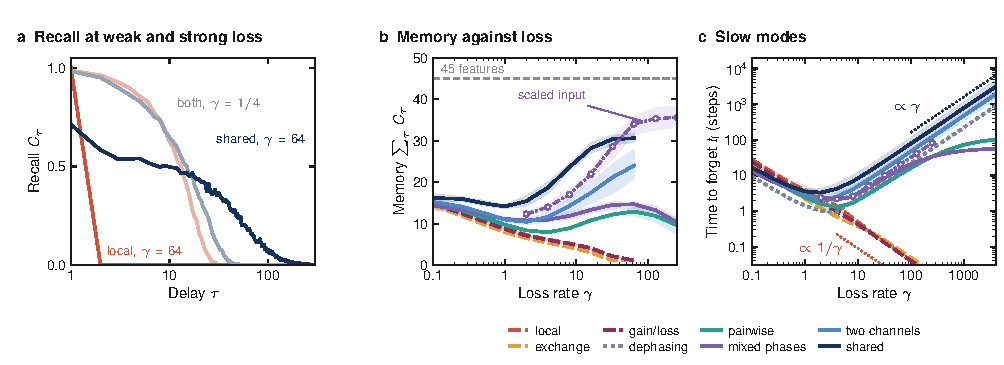
\includegraphics[width=\textwidth]{figures/fig2_families.pdf}
\caption{\textbf{The jump operators decide whether stronger dissipation erases or protects memory.}
Five-spin reservoirs at equal total coupling; lines and shading are the mean and the 16th--84th percentiles
over eight reservoirs.
\textbf{a}~Recall $C_\tau$ of the input $\tau$ steps back, for local loss and one shared channel at weak
($\gamma=1/4$, light) and strong ($\gamma=64$, dark) loss; mean over eight reservoirs.
\textbf{b}~Memory $\sum_\tau C_\tau$ for all jump families at a fixed input amplitude; one and two shared channels are
shown up to $\gamma=64$, beyond which their recall outgrows the 300 delays summed (Methods), mixed phases and pairwise
loss up to $\gamma=256$. Dash-dotted with circles, up to $\gamma=256$: mixed phases with the input amplitude scaled as
$\min(1,\gamma^{-1/2})$. Dashed: the limit of 45 set by the 45 features.
\textbf{c}~Time to forget, from the decay rates of the slow modes of the input-averaged step. Without protected
operators it falls as $1/\gamma$. With dark states it grows in proportion to $\gamma$ when the input cannot reach them
directly; with mixed phases and pairwise loss it levels off, unless the input amplitude is scaled down
(dash-dotted, mixed phases).
Dephasing protects populations into which the input never writes, so its memory in \textbf{b} is zero.}
\label{fig:families}
\end{figure*}

\subsection{Stronger dissipation, opposite consequences}
Figure~\ref{fig:families} shows the result. At weak dissipation all families behave alike, as the equal
coupling suggests (Fig.~\ref{fig:families}a,b). As $\gamma$ grows they split. With local loss, recall
retreats to ever shorter delays, until at $\gamma=64$ only the last input is left (Fig.~\ref{fig:families}a), and the
memory falls steadily (Fig.~\ref{fig:families}b). With a shared channel the memory dips and then, beyond
$\gamma\approx1$, doubles; at $\gamma=64$ recall reaches back more than a hundred steps. Exchange and gain/loss follow
local loss, and the split channel follows the shared one. Pairwise loss and mixed phases recover after a dip, but
only to their weak-dissipation level, and at stronger loss their memory falls again; we explain this difference
below.

The time to forget makes the split precise (Fig.~\ref{fig:families}c). We compute it from the slow modes of
the input-averaged step, the modes that the loss alone leaves untouched. Without protected operators it
falls as $1/\gamma$. With dark states it grows with $\gamma$. It keeps growing in proportion to $\gamma$ when the
input cannot reach the dark states directly (one shared channel, two channels); for one shared channel, $\gamma$
times the mean slow decay rate approaches about 3. When it can (mixed phases, pairwise loss), the input itself
scrambles the dark states, and the time to forget levels off, for pairwise loss only at larger $\gamma$ (Methods). Stronger loss slows forgetting only when the jump
operators leave dark states.

Dephasing shows what protection alone does not provide. Its 32 protected populations also forget ever more
slowly, yet its memory is zero at every $\gamma$: dephasing and the unitary input both leave the maximally mixed
state unchanged, and it is the unique stationary state for every input, so the reservoir relaxes to it whatever
the input. Protection is useful only for what the input can write into it. With exact features, recall counts
what is linearly recoverable however small the signal; we return to the size of the signal below.

\subsection{Dark states hold the memory}
Why does more loss help a shared channel? A strong channel acts like a continuous measurement of whether an
excitation has left, and such a measurement holds the state where the answer is
no~\cite{Beige2000,FacchiPascazio2002} (Fig.~\ref{fig:concept}c). To leading order in $1/\gamma$ the reservoir follows its Hamiltonian
projected onto the operators that the dissipator leaves alone, which turns the state but cannot forget.
Forgetting enters one order later, when the Hamiltonian briefly lifts a dark state into a bright one that
decays~\cite{Zanardi2014,Reiter2012}:
\begin{equation}
  \mathcal G(u)=\mathcal P\mathcal H(u)\mathcal P-\frac1\gamma\,\mathcal P\mathcal H(u)\mathcal S\mathcal H(u)\mathcal P ,
  \label{eq:reduced}
\end{equation}
with $\mathcal H=-i[H,\cdot\,]$, $\mathcal P$ the projector onto the protected operators and $\mathcal S$ the
inverse of the unit-rate dissipator on the rest (Methods). This is a rotation plus a leak of order $1/\gamma$:
an orthogonal map at the edge of stability, the classic recipe for long memory in a network~\cite{White2004}.
Equation~\eqref{eq:reduced} holds for any number of spins, so the leak falls as $1/\gamma$ at every size; the size
sets only its coefficient (Methods) and how strong the loss must be for this regime to begin.

Figure~\ref{fig:dark}a counts the protected operators of every family, and three tests confirm the picture.
At strong loss, 99 eigenvalues of the averaged step
approach the unit circle, one for each operator on the dark subspace apart from the stationary state; with
local loss they stay near zero (Fig.~\ref{fig:dark}b). The ten-state model of Eq.~\eqref{eq:reduced}, with
nothing fitted, reproduces the recall of the full reservoir from $\gamma\approx4$ on, within a few percent
(Fig.~\ref{fig:dark}c). Erasing the dark coordinates after every step removes all memory beyond a few
steps, while erasing a rotated copy of the same dimension leaves most of it (Fig.~\ref{fig:dark}d).

\begin{figure*}[t]
\centering
\includegraphics[width=\textwidth]{figures/fig3_dark.pdf}
\caption{\textbf{Dark states hold the memory.}
\textbf{a}~Number of operators that each unit-rate dissipator leaves unchanged, at five spins (open circle:
populations only).
\textbf{b}~Eigenvalues of the input-averaged step of one reservoir: one shared channel at $\gamma=1$, 8 and 64
(light to dark) and local loss at $\gamma=8$.
\textbf{c}~Recall of the full reservoir (lines) and of the dark-state model of Eq.~\eqref{eq:reduced} (circles),
with nothing fitted; mean of eight reservoirs.
\textbf{d}~Recall at $\gamma=16$ when the dark coordinates, or a copy of the dark subspace rotated by random
single-spin unitaries, are erased after every step; mean and 16th--84th percentiles over eight reservoirs.}
\label{fig:dark}
\end{figure*}

\subsection{The price of protection}
A long memory is not automatically a useful one. Every input turns the stored state a little, and the turn
depends on the input (Fig.~\ref{fig:concept}d). Over its memory time the stored direction thus takes a random
walk of steps $\pm\theta$ and spreads by about $\theta\sqrt{t_{\mathrm{mem}}}$. While the spread is small, the
measured projection is linear in each input. Once it reaches about a radian, the projection wraps around: the
record of an old input survives only multiplied by the inputs that followed it. A linear readout of a few
observables recovers single inputs; it cannot turn such products back into them. We call the number of distinct
inputs that a stored function involves its order, and we resolve the memory by
order~\cite{Dambre2012,MartinezPenaIPC2023} (Methods).

The simplest protected reservoir is reset to a fixed state with a small probability $p$ in each step and is
otherwise turned by an input-dependent unitary. The variance of a stored signal then decays over
$t_{\mathrm{mem}}=1/(2p)$ steps.
Write the step in traceless coordinates as an orthogonal map $O(u)$ and call $s=1-\|\mathbb EO\|_F^2/n$ the mixing
fraction of one input. It is the mean squared fraction of a randomly oriented state that one input moves away from
the average turn, and it grows as the square of the input amplitude for small turns.

\begin{theorem}[Mixing law]\label{thm:law}
Let a reservoir be reset with probability $p$ per step and otherwise turned by input-dependent rotations that
mix the stored state and write a signal (conditions in Appendix~\ref{app:law}). Draw the order $D_p$ of a stored
function with probability equal to its share of the memory. As $p\to0$, $pD_p$ becomes exponentially distributed,
with mean
\begin{equation*}
  \mathbb ED_p=s\,t_{\mathrm{mem}}+O(1).
\end{equation*}
\end{theorem}

In words, a memory mixes on average $s\,t_{\mathrm{mem}}$ inputs, the mixing fraction times the memory time.
Halving the reset probability doubles the typical order, and any fixed set of orders carries a vanishing share
of the memory although its total stays constant (Appendix~\ref{app:law}). In a protected reservoir the leakage
plays the role of $p$, so a fixed input amplitude makes memory mix more and more inputs as the loss grows.

Mixing is not only a cost. Products of inputs are the nonlinear memory that tasks such as parity
need~\cite{Dambre2012,Inubushi2017}, and the mixing law says how many inputs a reservoir combines. In the first version of
this study the equal-phase shared channel scored below local loss on parity and closed-loop
forecasting~\cite{BaumannV1} (Appendix~\ref{app:v1}). This is consistent with its input having no matrix element
between its dark states (Sec.~\ref{sec:writing}): at $\gamma=1$ its readout recovers half as much capacity of polynomial
degree three and four as that of local loss, while with mixed phases, where the input reaches the dark states
directly, it recovers as much as with local loss (Methods).

\subsection{How strongly to write}
\label{sec:writing}
Mixing is not the only cost of a large input amplitude. A single qubit that relaxes towards $+X$ at rate $\epsilon$, is
turned about $Z$ by $\pm\theta$ per input and is read along $Y$ shows the whole trade-off in closed form
(Fig.~\ref{fig:writing}a, Appendix~\ref{app:qubit}). Everything depends on $\theta^2/\epsilon$, the squared turn per
memory time. For large values the inputs mix, and they also scramble the polarization that each new input tilts,
so the stored signal shrinks. For small values each input writes too little. The stored signal is largest at
$\theta^2/\epsilon=2/\sqrt3$. Both results follow one rule: keep the mixing fraction times the memory time of order
one. With $s\propto\theta^2$ and $t_{\mathrm{mem}}\propto1/\epsilon$ this means $\theta^2\propto\epsilon$: the input
amplitude must fall as the square root of the leakage.

\begin{figure}[!tb]
\centering
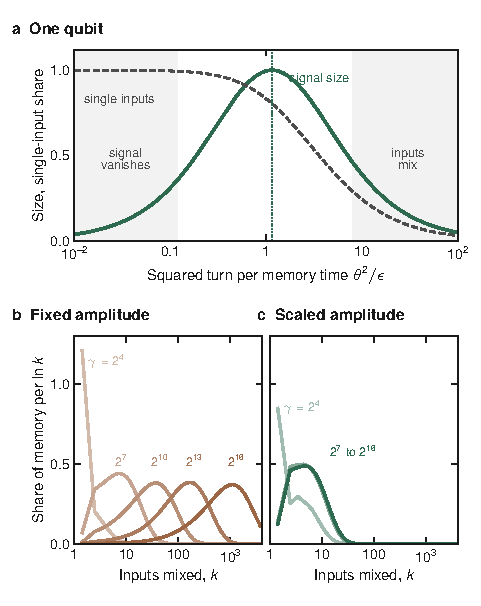
\includegraphics[width=\columnwidth]{figures/fig4_writing.pdf}
\caption{\textbf{How strongly to write into a protected reservoir.}
\textbf{a}~One qubit relaxing at rate $\epsilon$ and turned by $\pm\theta$ per input, in the limit $\epsilon\to0$ at
fixed $\theta^2/\epsilon$: size of the stored signal (normalized to its maximum at $\theta^2/\epsilon=2/\sqrt3$, dotted)
and share of single past inputs (dashed).
\textbf{b,c}~Three-spin reservoir with one shared channel of mixed phases (Hamiltonian H3): share of the memory of
$X_1$ carried by products of $k$ inputs, per unit $\ln k$, at $\gamma=2^4$, $2^7$, $2^{10}$, $2^{13}$ and $2^{16}$ (light
to dark), for a fixed input amplitude (b) and for an amplitude scaled as $8/\sqrt\gamma$ (c).}
\label{fig:writing}
\end{figure}

The jump operators decide how strongly an input reaches the protected space. The dark states of a shared
channel $L\propto\sum_ic_i\sigma_i^-$ are annihilated by $\sum_ic_i\sigma_i^-$. An input field $\sum_ic_iX_i$ along
the same phase vector is the sum of this operator and its adjoint, so it has no matrix element between dark
states. It writes only through brief excursions into bright states, and its effect falls as $1/\gamma$, while an
input pattern across the phase vector reaches the dark states directly (Methods). This explains the families of
Fig.~\ref{fig:families}. The uniform input of Eq.~\eqref{eq:H} lies along the phases of the equal-phase channel and
of each split channel, so it reaches the dark states only through bright states: their memory grows with the loss,
but the signal behind it shrinks.
For mixed phases and for pairwise loss the same input reaches the dark states directly. Their records are mixed
by later inputs, so the memory of single inputs stays near its weak-dissipation level and falls at the strongest
loss. Scaling the input amplitude
down as $\gamma^{-1/2}$ removes this limit (dash-dotted in Fig.~\ref{fig:families}b,c): with mixed phases the memory
then grows with the loss like that of the shared channel, the time to forget grows in proportion to $\gamma$ again,
and at strong loss the signal in each feature keeps a roughly constant size (Methods). The memory cannot exceed 45, one unit per feature.
It levels off near 36, and as the time to forget keeps growing each delay is recalled more weakly: the memory becomes
longer, not larger.

A three-spin reservoir with one shared channel of mixed phases, whose protected space the input reaches
directly, shows both limits (Methods). With a fixed input amplitude the order of its memory grows in proportion to
$\gamma$ and single inputs lose their share (Fig.~\ref{fig:writing}b), while the signal in a measured spin shrinks as
$1/\gamma$. With the amplitude scaled as $8/\sqrt\gamma$, which exceeds the fixed amplitude below $\gamma=64$ and
falls below it above, the order stays small (Fig.~\ref{fig:writing}c), single inputs keep a finite share, the
signal stays finite, and the range of delays that holds 90\% of the single-input recall grows in proportion to
$\gamma$. Here a single observable holds at most one unit of memory, so as the range grows each delay is recalled
more weakly, roughly as $1/\gamma$. We prove both limits for four Hamiltonians and
for neighbourhoods of their couplings with computer-assisted bounds (Appendix~\ref{app:spins}).

Which part of the protected state carries this memory? Coherence is known to shape the performance of spin
reservoirs~\cite{Palacios2024}; here we isolate its role. We return the spins to the dark subspace after every
input and compare two arms that differ only in a dephasing of the dark energy levels. The populations follow the
same slow dynamics in both arms, but without coherence the stored signal collapses as $1/\gamma^2$ (Methods). A new
input first turns a population into a coherence, and erasing the coherences deletes each record as soon as it is
written (Appendix~\ref{app:spins}).
